\documentclass{beamer}
\usecolortheme{wolverine}

% math stuff
\usepackage{amsmath}
\usepackage{amsthm}
\usepackage{amssymb}
\usepackage{xcolor}

\usepackage{float}
\usepackage{subcaption}

% to insert images
\usepackage{graphicx}

% to correctly insert stressed characters
\usepackage[T1]{fontenc}
\usepackage[utf8]{inputenc}

\usepackage{multirow}

% Bibliography
% \usepackage[style=alphabetic]{biblatex}
% \usepackage[nottoc]{tocbibind}
% \usepackage{bibentry}
% \setcounter{biburllcpenalty}{9000}
% \usepackage{nameref}

% to put links in table of contents
\usepackage{hyperref}
\hypersetup{colorlinks=false, %set true if you want colored links
    linktoc=all,     %set to all if you
}

% Add symbols
% \usepackage{textcomp}

% Add command for Real and Z sets
% \usepackage{dsfont}
% \newcommand{\Rset}{$\mathds{R}$}
% \newcommand{\Zset}{$\mathds{Z}$}

% Code highlighting
% \usepackage{minted}
% \usemintedstyle{perldoc}
% \setminted{
%     frame=single,
%     breaklines,
% }

% tikz figures
% \usepackage{tikz}
% \input{style.tikzstyle}
% \usetikzlibrary{positioning}

% number rounding
\usepackage{siunitx}
\sisetup{round-mode=places,round-precision=5}

\definecolor{myyellow}{RGB}{225, 225, 0}

\begin{document}
\title{Thesis notes}
\date{2nd March}
\frame{\titlepage}

\begin{frame}[c]
    \frametitle{A user-content graph on r/AskTrumpSupporters}
    \begin{figure}[htpb]
        \centering
        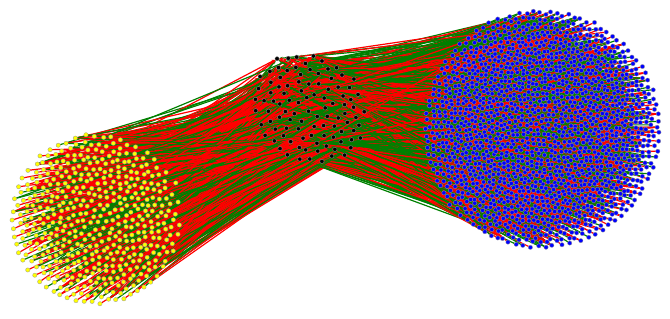
\includegraphics[width=0.8\linewidth]{img/experimental-graph.png}
        \caption{A graph built on 200 contents from r/AskTrumpSupporters, with
        \textcolor{myyellow}{Supporters}, \textcolor{blue}{Non
    Supporters} and Content nodes}%
        \label{fig:img/experimental-graph}
    \end{figure}
\end{frame}

\begin{frame}[c]
    \frametitle{Measuring content separation (1)}
    \begin{tabular}{l|l|c|c|}
        \multicolumn{2}{c}{}&\multicolumn{2}{c}{User label}\\
        \cline{3-4}
        \multicolumn{2}{c|}{}&Supporter&Non Supporter\\
        \cline{2-4}
        \multirow{2}{*}{Stance}& Positive & $a$ & $b$ \\
        \cline{2-4}
                                       & Negative & $c$ & $d$ \\
                                       \cline{2-4}
    \end{tabular} 

    \bigskip

    If $a + d >> c + b$ then the content is close to \textcolor{blue}{supporters}.

    \bigskip

    If instead $c + b >> a + d$ then the content is close to
    \textcolor{myyellow}{non supporters}.

    \bigskip

    If $c + b \approx a + d$ then the content is neutral.
\end{frame}

\begin{frame}[c]
    \frametitle{Measuring content separation (2)}

    A possible measure of content separation:

    \begin{equation}
        \alpha = \frac{a + d}{a + b + c + d} 
    \end{equation}

    \begin{figure}[htpb]
        \centering
        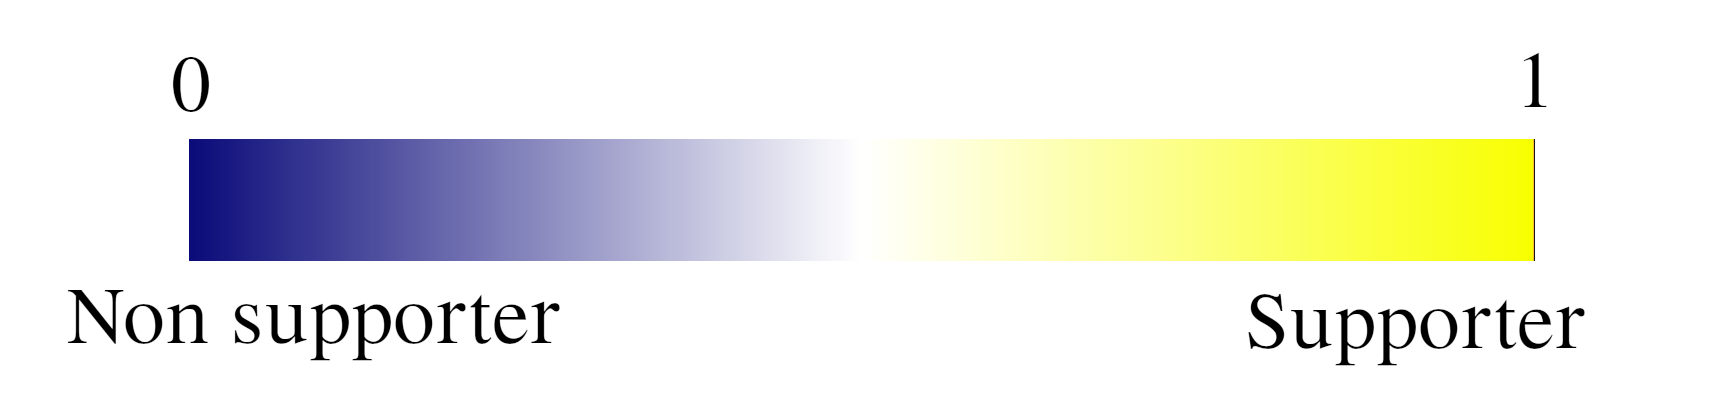
\includegraphics[width=0.8\linewidth]{img/gradient-caption.png}
        % \caption{img/gradient-Caption}%
        % \label{fig:img/gradient-caption}
    \end{figure}

\end{frame}

\begin{frame}[c]
    \frametitle{Measuring content separation (3)}

    \begin{figure}[htpb]
        \centering
        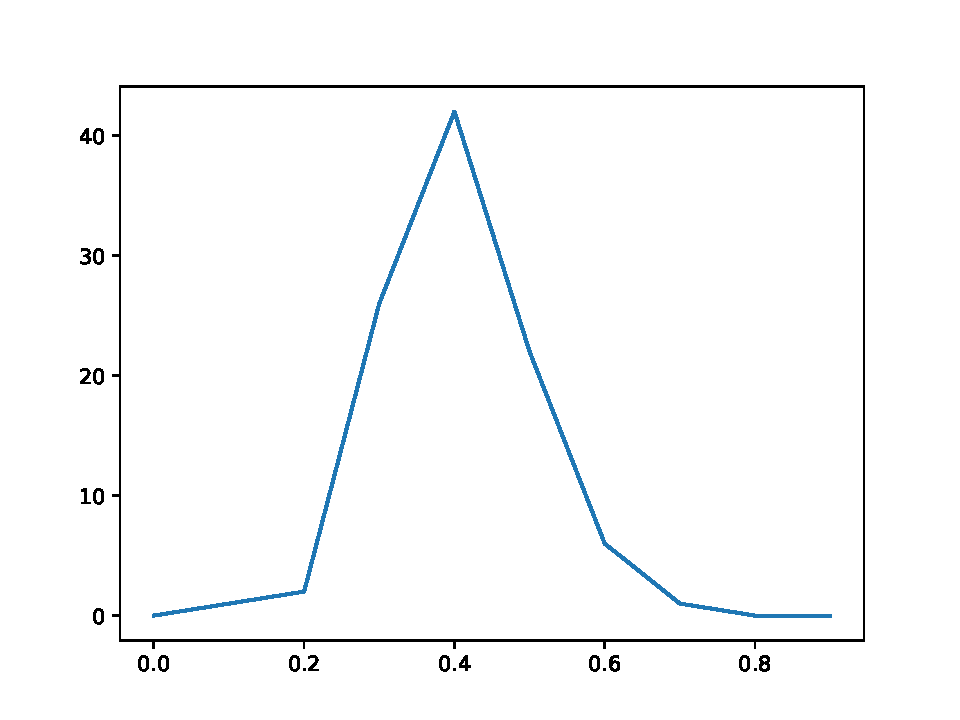
\includegraphics[width=0.8\linewidth]{out/experimental200/experimental200-support-hist.pdf}
        \caption{Histogram of content per $\alpha $}%
        \label{fig:out/experimental200/experimental200-support-hist}
    \end{figure}
\end{frame}

\begin{frame}[c]
    \frametitle{A larger graph from @nytimes (1)}
    \begin{figure}[htpb]
        \centering
        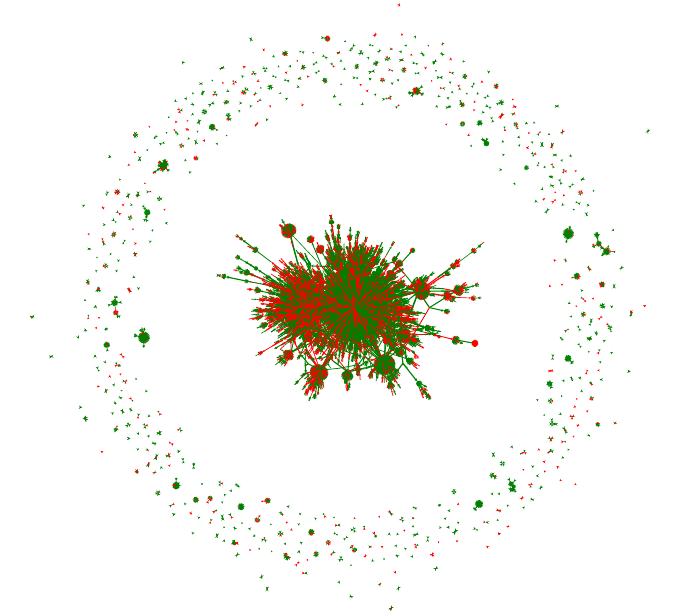
\includegraphics[width=0.7\linewidth]{img/nytimes-graph.png}
        \caption{A graph built on 400 contents from @nytimes}%
        % \label{fig:img/nytimes-graph}
    \end{figure}
\end{frame}

\begin{frame}[c]
    \frametitle{A larger graph from @nytimes (2)}
    \begin{itemize}
        \item The graph has 15914 vertices and 26439 edges
        \item Fraction of negative edges: \num{0.44245243768675063}
        \item Clustering coefficient: \num{0.0006692190839971315} with standard
            deviation \num{0.02023216899947087}
        \item Average shortest path length: \num{13.534551279796096}
        \item Median shortest path length: 14.0
        \item Average degree: \num{3.3227346990071633}
        \item Unique average degree: \num{2.2842779942189266}
    \end{itemize}
\end{frame}

\begin{frame}[c]
    \frametitle{A larger graph from @nytimes (3)}
    \begin{figure}[htpb]
        \centering
        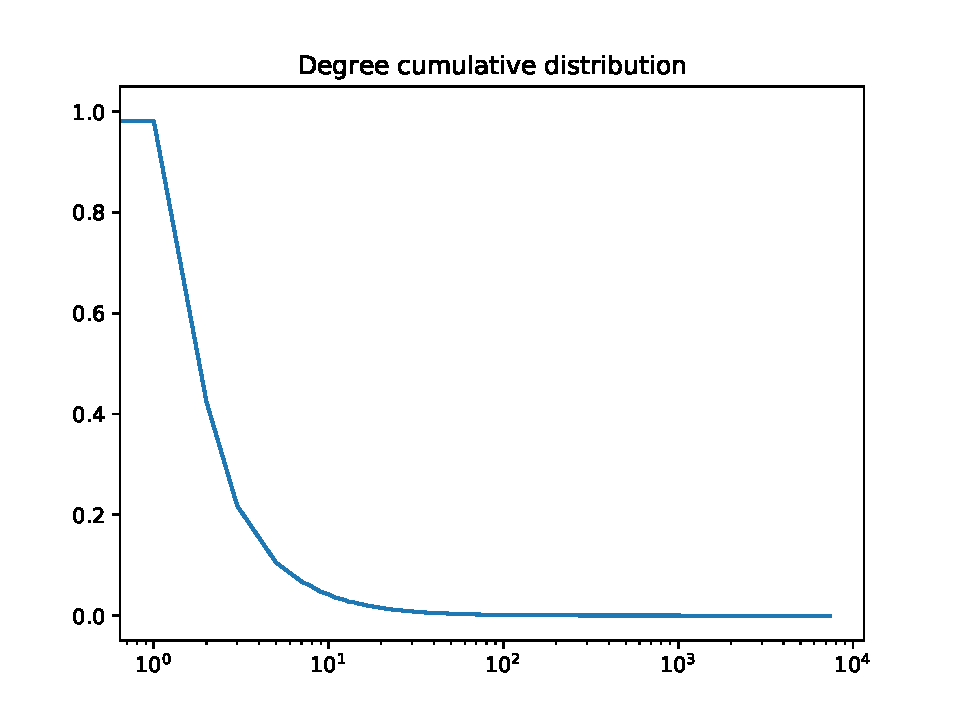
\includegraphics[width=0.8\linewidth]{out/nytimes400/nytimes400-degree-dist.pdf}
        \caption{Cumulative degree distribution (log scale)}%
    \end{figure}
\end{frame}

\begin{frame}[c]
    \frametitle{A larger graph from @nytimes (4)}
    \begin{figure}[htpb]
        \centering
        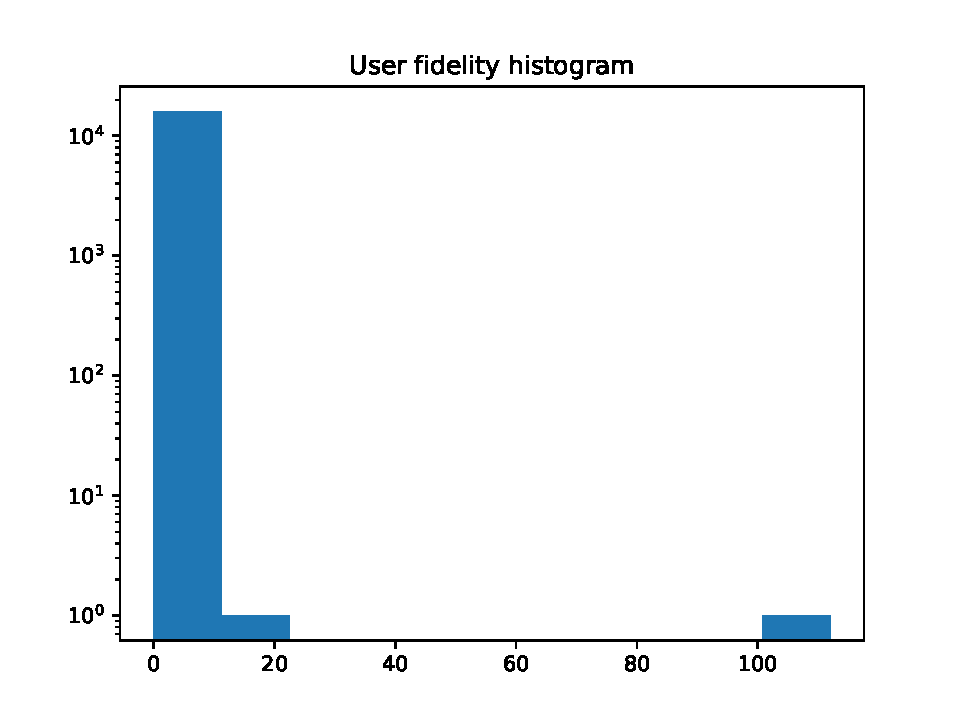
\includegraphics[width=0.8\linewidth]{out/nytimes400/nytimes400-fidelity-hist.pdf}
        \caption{Histogram of users per number of contents they discussed}%
    \end{figure}
\end{frame}

\begin{frame}[c]
    \frametitle{A larger graph from @nytimes (5)}
    \begin{figure}[htpb]
        \centering
        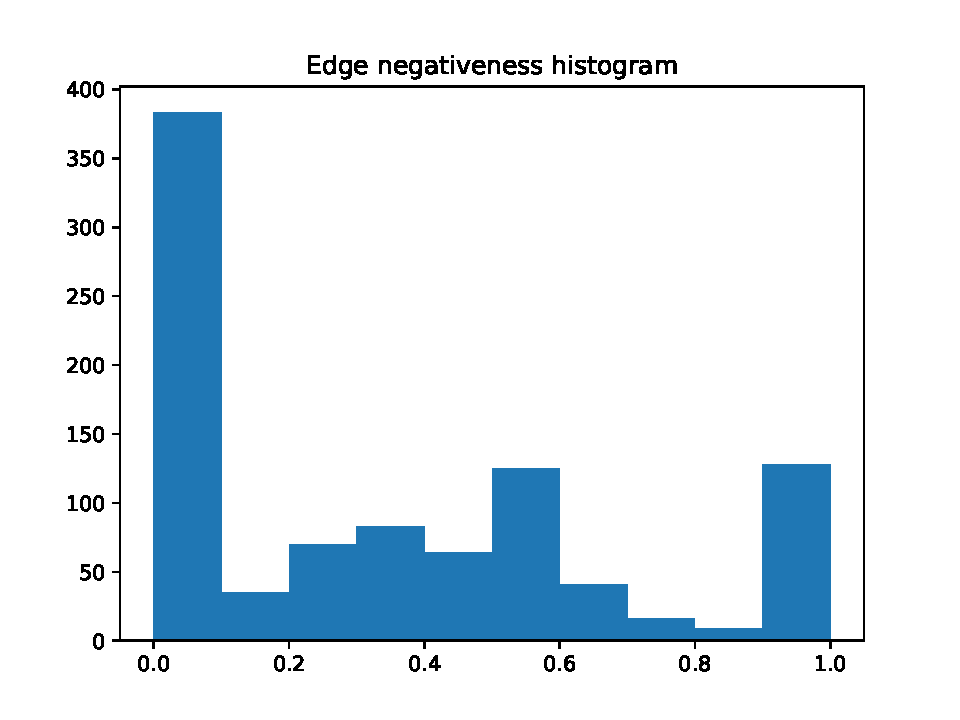
\includegraphics[width=0.8\linewidth]{out/nytimes400/nytimes400-neg-fraction-hist.pdf}
        \caption{Histogram of contents per fraction of negative edges}%
    \end{figure}
\end{frame}

\begin{frame}[c]
    \frametitle{A larger graph from @foxnews (1)}
    \begin{figure}[htpb]
        \centering
        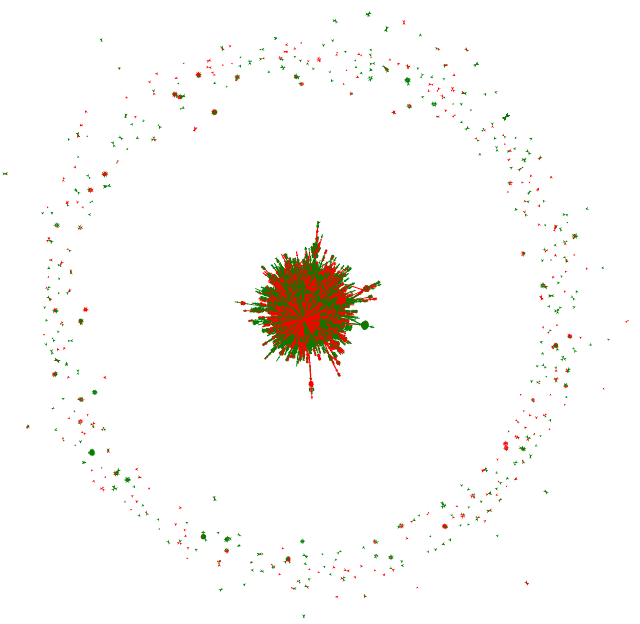
\includegraphics[width=0.7\linewidth]{img/foxnews-graph.png}
        \caption{A graph built on 400 contents from @foxnews}%
        % \label{fig:img/foxnews-graph}
    \end{figure}
\end{frame}

\begin{frame}[c]
    \frametitle{A larger graph from @foxnews (2)}
    \begin{itemize}
        \item The graph has 41188 vertices and 158540 edges
        \item Fraction of negative edges: \num{0.5650687523653337}
        \item Clustering coefficient: \num{0.0007972611178168763} with standard
            deviation \num{0.26148580937513294}
        \item Average shortest path length: \num{7.1590701507576515}
        \item Median shortest path length: 7.0
        \item Average degree: \num{7.698358745265612}
        \item Unique average degree: \num{2.6409148295620084}
    \end{itemize}

\end{frame}

\begin{frame}[c]
    \frametitle{A larger graph from @foxnews (3)}
    \begin{figure}[htpb]
        \centering
        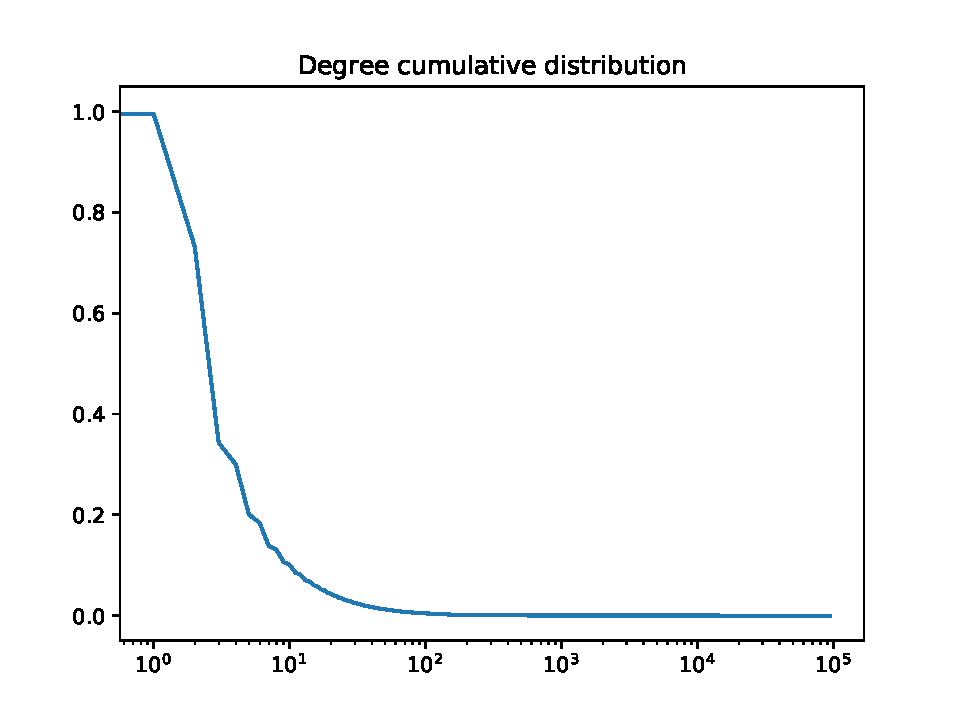
\includegraphics[width=0.8\linewidth]{out/foxnews400/foxnews400-degree-dist.pdf}
        \caption{Cumulative degree distribution (log scale)}%
    \end{figure}
\end{frame}

\begin{frame}[c]
    \frametitle{A larger graph from @foxnews (4)}
    \begin{figure}[htpb]
        \centering
        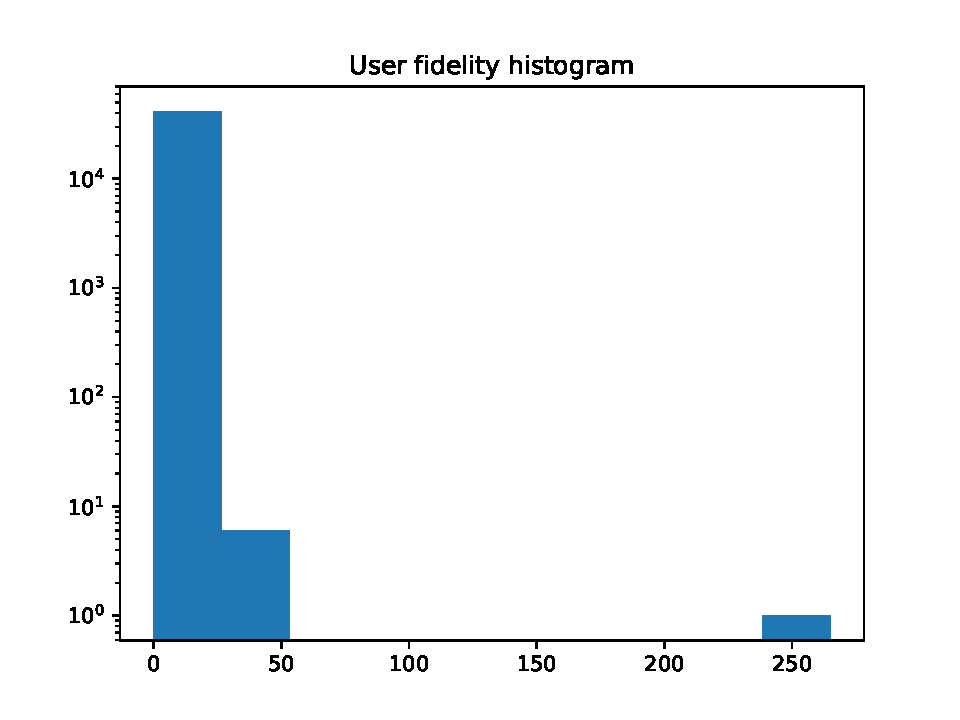
\includegraphics[width=0.8\linewidth]{out/foxnews400/foxnews400-fidelity-hist.pdf}
        \caption{Histogram of users per number of contents they discussed}%
    \end{figure}
\end{frame}

\begin{frame}[c]
    \frametitle{A larger graph from @foxnews (5)}
    \begin{figure}[htpb]
        \centering
        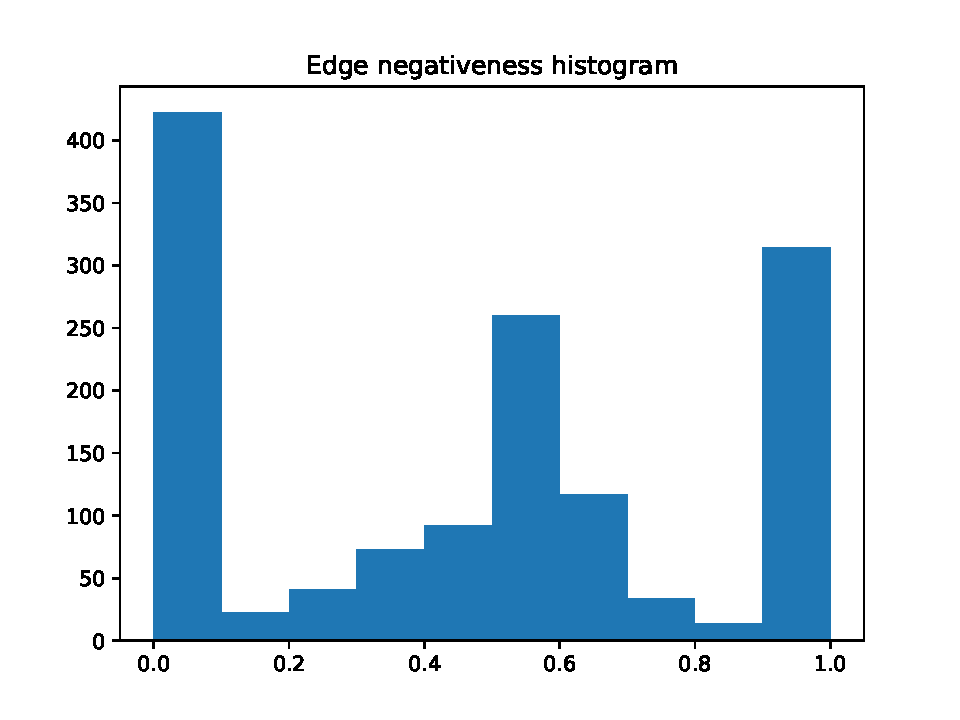
\includegraphics[width=0.8\linewidth]{out/foxnews400/foxnews400-neg-fraction-hist.pdf}
        \caption{Histogram of contents per fraction of negative edges}%
    \end{figure}
\end{frame}

\end{document}


